\documentclass[conference,comsoc,twoside,caption=false]{IEEEtran}
\usepackage[T1]{fontenc}
\usepackage{newtxtext,newtxmath}
\ifCLASSOPTIONcompsoc
  \usepackage[caption=false,font=footnotesize,labelfont=sf,textfont=sf]{subfig}
\else
  \usepackage[caption=false,font=footnotesize,labelfont=small]{subfig}
\fi
\captionsetup[figure]{font=footnotesize}
\ifCLASSOPTIONcaptionsoff
  \usepackage[nomarkers]{endfloat}
  \let\MYoriglatexcaption\caption
  \renewcommand{\caption}[2][\relax]{\MYoriglatexcaption[#2]{#2}}
\fi
\usepackage[utf8]{inputenc}
\usepackage{ragged2e}
\usepackage{graphicx}
\usepackage{listings}
\lstdefinestyle{promptstyle}{%
  basicstyle=\ttfamily\scriptsize,
  frame=single,
  framesep=3pt,
  breaklines=true,
  breakindent=0pt,
  columns=fullflexible,
  keepspaces=true,
  showstringspaces=false,
  aboveskip=2pt,
  belowskip=2pt,
  xleftmargin=3pt,
  xrightmargin=3pt,
}
\usepackage{tabulary}
\usepackage{booktabs}
\usepackage{mathtools}
\let\openbox\relax
\usepackage{amsmath}
\usepackage{amsthm}
\let\Bbbk\relax
\usepackage{amssymb}
\usepackage{amsfonts}
\interdisplaylinepenalty=2500
\usepackage[noadjust]{cite}
\usepackage{balance}
\usepackage{tabularx}
\usepackage{comment}
\usepackage{setspace}
\usepackage{xspace}
\usepackage{acronym}
\usepackage{multirow}
\usepackage{upgreek}
\usepackage{nicefrac}
\usepackage{ifthen}
\usepackage[bookmarks=false]{hyperref}
\hypersetup{draft}
\usepackage{caption}
\usepackage{cleveref}
\usepackage[inline]{enumitem}
\usepackage{makecell}
\usepackage{siunitx}
\usepackage{placeins}
\renewcommand{\baselinestretch}{0.877}
\theoremstyle{definition}
\newtheorem{exmp}{Example}
\DeclareMathOperator{\Expectation}{\mathbb{E}\xspace}
\DeclareMathOperator{\Probability}{\mathbb{P}\xspace}
\usepackage[table]{xcolor}
\usepackage{flushend}

\acrodef{NTN}{Non-Terrestrial Network}
\acrodef{MEC}{Multi-Access Edge Computing}
\acrodef{LEO}{Low Earth Orbit}
\acrodef{DRL}{Deep Reinforcement Learning}
\acrodef{LLM}{Large Language Model}
\acrodef{SLM}{Small Language Model}
\acrodef{SoC}{State of Charge}
\acrodef{ISL}{Inter-Satellite Link}
\acrodef{IoT}{Internet of Things}
\acrodef{KPI}{Key Performance Indicator}
\acrodef{NPU}{Neural Processing Unit}
\acrodef{MLP}{Multi-Layer Perceptron}
\acrodef{GDPR}{General Data Protection Regulation}
\acrodef{RAM}{Random-Access Memory}
\acrodef{API}{Application Programming Interface}
\acrodef{CI}{Confidence Interval}
\acrodef{IQR}{Interquartile Range}
\acrodef{RAPL}{Running Average Power Limit}

\hyphenation{al-go-rithm allows op-tical net-works semi-conduc-tor ubi-quitous
energy expe-riments satel-lite con-stel-lation orches-tration se-mantic
com-pliance}

\begin{document}
\author{
\IEEEauthorblockN{Oct\'{a}vio B. Nascimento and Carlos A. Astudillo}
\IEEEauthorblockA{%
Institute of Computing, State University of Campinas (UNICAMP),
Campinas, SP, 13083-852, Brazil\\
Emails: o241327@dac.unicamp.br, castudillo@unicamp.br}
}
\title{\huge Semantic Task Orchestration in LEO-NTN\\
Multi-Access Edge Computing:
A Comparative Study}
\maketitle
    \newcommand{\MYheader}{\smash{\scriptsize
    \hfil\parbox[t][\height][t]{\textwidth}{\centering {}}\hfil\hbox{}}}
    \makeatletter
    \def\ps@IEEEtitlepagestyle{%
    \def\@oddhead{\MYheader}%
    \def\@evenhead{\MYheader}%
    \def\@oddfoot{}%
    \def\@evenfoot{}}
    \makeatother
    \pagestyle{headings}
    \addtolength{\footskip}{0\baselineskip}
    \addtolength{\textheight}{-0.1\baselineskip}
\begin{abstract}
\ac{MEC} over \ac{LEO} constellations introduces extreme constraints on task orchestration, including tight energy budgets driven by orbital eclipses, high-dynamic system topology, 
bounded decision windows, and heterogeneous computing payloads.
Beyond classical resource management, real-world tasks increasingly carry
\emph{semantic constraints} that pure numerical optimizers cannot interpret, including data sovereignty laws, privacy regulations, and
hardware-failure protocols. 
This work presents a controlled comparative simulation of four orchestration
paradigms over the same 1{,}200-second scenario and identical 69-task workload:
(i)~a greedy heuristic baseline, (ii)~a \ac{DRL} agent (SB3 DQN,
50{,}000~training steps), (iii)~a \ac{SLM} simulating on-device \ac{NPU}
inference (Gemma~4 26B, \SI{50}{\milli\second} benchmark latency), and
(iv)~a \ac{LLM} cloud orchestrator (Gemini~3.1 Flash~Lite). The LLM attains full anomaly compliance (8/8; Wilson 95\%~CI 67.6--100\%)
against 25\% for the heuristic ($p=0.031$, exact paired McNemar). A rule table,
or a DRL agent given the rule type, matches it on these design-time rules; the
difference emerges on unseen constraints stated in natural language, where the
LLM keeps 20/20 while the rule table collapses to the heuristic and the SLM to a
discard reflex. Decision energy, under a declared model, is orders of magnitude
higher for the LLM yet negligible against the battery budget: the operative cost
of semantic compliance is latency and dependence on a ground link.
\end{abstract}
\begin{IEEEkeywords}
NTN-MEC, LEO satellite edge computing, deep reinforcement learning,
large language models, semantic compliance, task orchestration.
\end{IEEEkeywords}
\acresetall
\IEEEpeerreviewmaketitle

\section{Introduction}
\label{sec:intro}

The proliferation of \ac{LEO} constellations has positioned satellite nodes
as candidates for \ac{MEC} infrastructure. When a constellation acts as a
compute fabric, each satellite must independently decide, in real time, whether
to accept an incoming processing task, redirect it to a peer via \ac{ISL}, or
discard it---all subject to strict battery and memory constraints imposed by the
orbital eclipse cycle~\cite{guo2024,gpp2022}.

Beyond classical resource constraints, an emerging class of tasks carries
semantic constraints derived from real-world regulations: data privacy laws
(e.g., \ac{GDPR}), national data sovereignty requirements, or hardware-level failure
protocols. A compliant orchestrator must parse these constraints from natural
language descriptions and map them onto routing decisions---a capability that
pure numerical optimizers fundamentally lack.

\ac{DRL}, and in particular the value-based Deep Q-Network (DQN) family
introduced by Mnih \emph{et al.}~\cite{mnih2015}, has been applied to satellite
MEC scheduling with promising results. Jiang \emph{et al.}~\cite{jiang2025}
propose a multi-agent DRL framework for on-orbit task scheduling, reporting
improvements of up to 70\% in completion time and 68\% in energy consumption
over unoptimized baselines. Closer to our setting, Casas \emph{et al.}~\cite{casas2026}
address DDQN-based routing in \ac{LEO} constellations and show that agent
performance hinges critically on the reward function, whose design remains a
manual, expertise-intensive process---so much so that they automate it with an
LLM-in-the-loop framework, underscoring the practical cost of reward
engineering. While computationally efficient, such DRL agents operate as
black-boxes over numerical feature vectors, making them unable to interpret
task-level semantic rules without explicit feature engineering.

\acp{LLM} have recently been explored for resource allocation in wireless
systems. Lee and Park~\cite{lee2024} demonstrate that LLMs can perform resource
allocation in wireless networks and explicitly propose a hybrid architecture---a
lightweight DNN for routine decisions combined with an LLM for complex semantic
cases---to compensate for LLM latency limitations, directly motivating the
DRL-vs-LLM trade-off this paper quantifies empirically. Abgaryan
\emph{et al.}~\cite{abgaryan2024} show that LLMs match specialised RL/GNN
approaches in job-shop scheduling benchmarks, confirming that LLM scheduling
capability is not merely a surface-level linguistic effect. The concept of
Edge Intelligence~\cite{deng2020} further motivates embedding compact language
models directly on edge nodes, blurring the boundary between \emph{AI for the
edge} and \emph{AI at the edge}.

For real LEO constellations, Shenoy \emph{et al.}~\cite{shenoy2024} demonstrate
with the CosMAC system that topology-aware scheduling for \ac{IoT} picosat
constellations achieves up to 6.5$\times$ throughput improvement over standard
MAC approaches, confirming that context-sensitive scheduling decisions have
measurable operational impact beyond simulation.

\textbf{Identified gap:} the literature treats DRL, LLM, and Edge Intelligence
as separate threads, each optimising a single numerical metric (time, energy,
throughput). No prior work directly compares all four paradigms---fixed
heuristic, DRL, embedded \ac{SLM}, and centralized LLM---in the same simulated
environment with primary focus on \emph{semantic compliance} rather than
throughput alone. This paper fills that gap with the following contributions:
\begin{enumerate}
  \item A multi-engine comparative simulation framework (4 paradigms,
    deterministic 1{,}200-second window, 69 identical tasks) enabling fair
    paradigm comparison under identical orbital conditions.
  \item A DRL agent trained with SB3 DQN over 50{,}000 synthetic steps using
    hidden-anomaly reward shaping, reaching 37.5\% anomaly compliance without
    observing semantic rule types. We show analytically that a binary-flag
    observation space caps expected compliance at $1/3$---the three rule types
    are equiprobable and only the mandatory-discard one is identifiable from a
    single bit---and verify over 20 seeds that the agent sits at that bound
    (29.0\%, 95\%~CI 22.1--37.0). The limit is therefore the observation space,
    not DRL as a paradigm nor the training budget.
  \item An information-parity evaluation: a rule table and a DRL agent given
    the rule type match the LLM on design-time constraints, but on unseen
    natural-language constraints only the LLM retains full compliance, while the
    SLM behaves as a discard reflex. All contrasts are reported with paired
    tests and interval estimates.
  \item An explicit \emph{parameter provenance audit} (Table~\ref{tab:params}):
    every simulation parameter is labelled either as grounded in cited
    literature or as a deliberate design choice, so that readers can separate
    externally validated premises from modelling decisions.
\end{enumerate}

\section{System Model}
\label{sec:sysmodel}

\begin{figure}[!t]
\centering
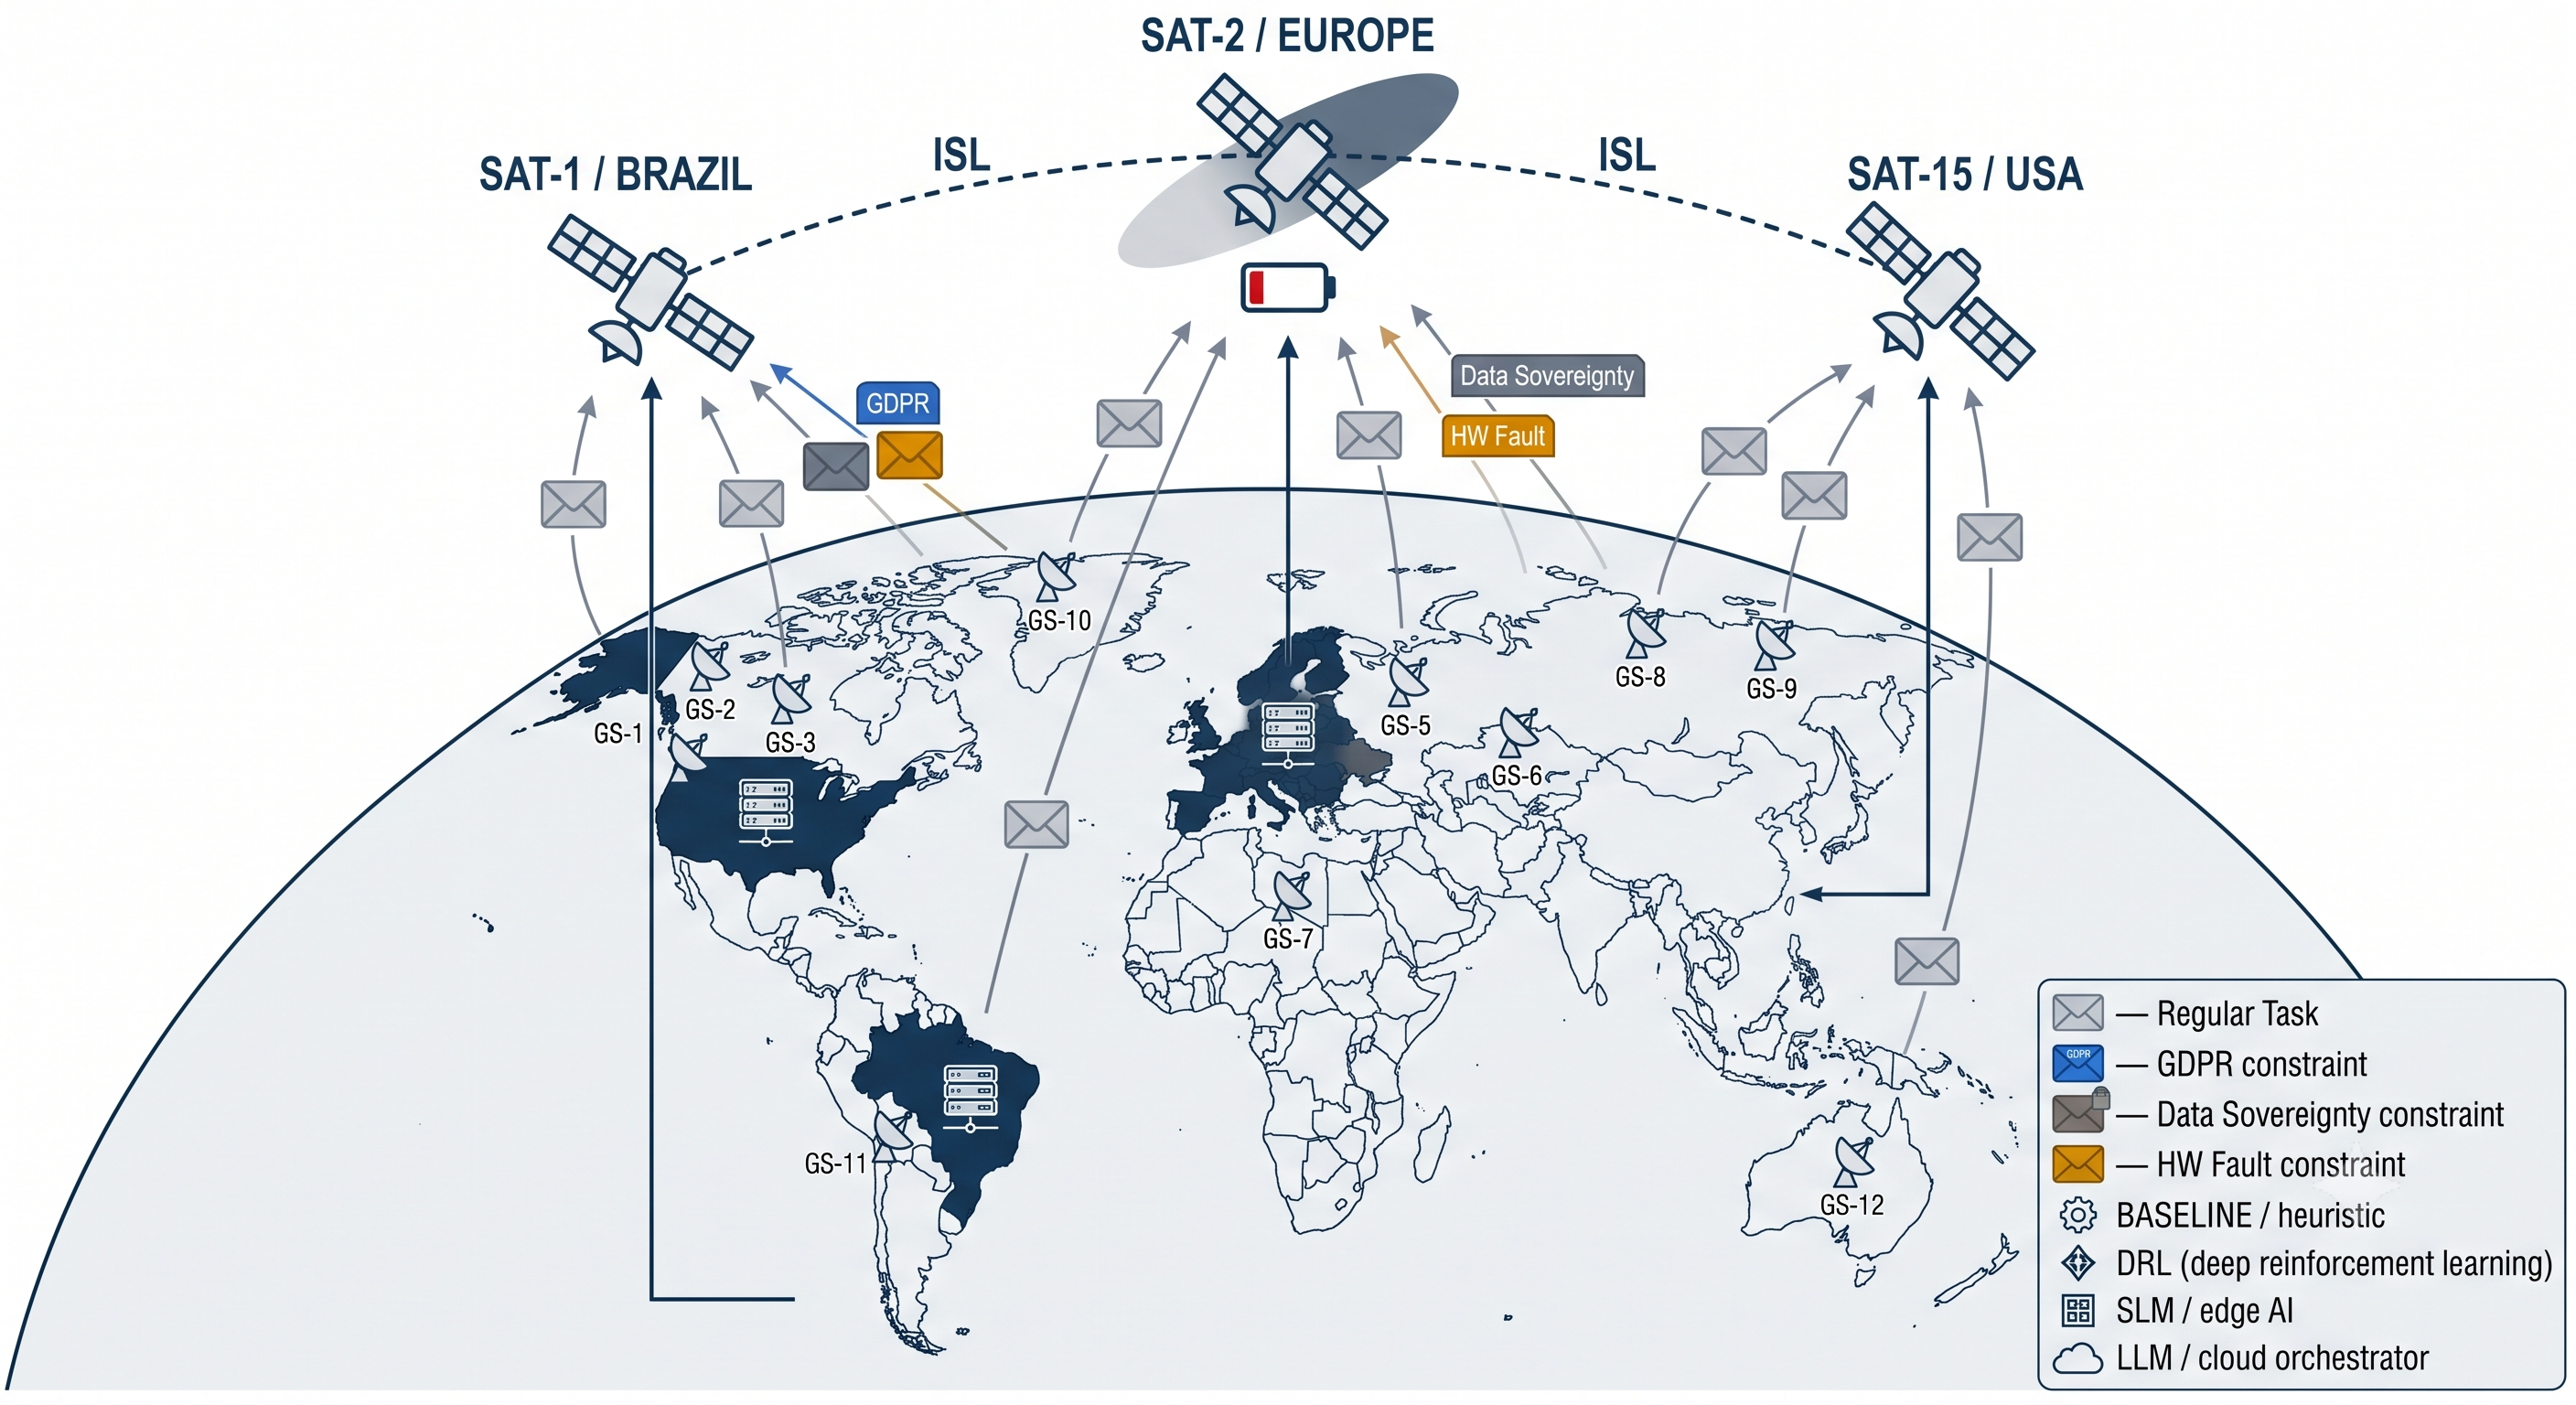
\includegraphics[width=\columnwidth]{architecture-diagram.png}
\caption{NTN-MEC orchestration architecture. Three regional \ac{LEO}-\ac{MEC}
nodes (Brazil, Europe, USA) receive a Poisson stream of tasks, each carrying a
region, a RAM requirement, and an optional semantic annotation. A pluggable
orchestration engine---BASELINE, DRL, SLM, or LLM---observes the real-time
satellite state (battery \ac{SoC}, free RAM, solar phase) and maps every task
onto one of four routing actions (SAT-1, SAT-2, SAT-15, or DROP) subject to
battery, memory, and semantic constraints.}
\label{fig:architecture}
\end{figure}

\subsection{Network Architecture}
Fig.~\ref{fig:architecture} depicts the overall orchestration architecture.
A constellation of three \ac{LEO} satellites operates as \ac{MEC} nodes, each
assigned to a fixed geographic region (Brazil, Europe, USA). Satellites carry
heterogeneous computational payloads: 4{,}096~MB RAM each, with battery
capacities of 75~Wh (SAT-1/Brazil), 50~Wh (SAT-2/Europe), and 100~Wh
(SAT-15/USA). These capacities are nominal: \ac{SoC} dynamics are expressed in
percentage points and do not scale with capacity, so the satellites differ in
initial \ac{SoC} (90/75/85\%) and orbital phase rather than in energy storage. The \ac{ISL} is assumed always available (a common assumption for
constellations with optical ISL), so drops reflect exclusively battery/RAM
exhaustion or semantic rule violations---never link failure.

\subsection{Task Arrival and Semantic Anomalies}
Task arrivals are drawn from a Poisson process with nominal rate
$\lambda = 4$~tasks/min, the standard model for aggregated \ac{IoT}/NTN
traffic~\cite{guo2024}, resolved on the 5-s simulation step: at most one task
arrives per step, and the next arrival is timed from the step that serves the
previous one. Inter-arrival times are thus $5\lceil X/5\rceil$~s with
$X\sim\mathrm{Exp}(\lambda)$, an effective rate of $\approx$3.4~tasks/min
(mean 17.6~s). Each task
requires 500~MB of RAM held for 60~seconds. A fraction $\alpha = 10\%$ of tasks
carry one of three semantic constraints, assigned uniformly at random:
(i)~\emph{GDPR compliance} (must route exclusively to EUROPE, or discard);
(ii)~\emph{data sovereignty} (must route exclusively to BRAZIL);
(iii)~\emph{critical hardware failure} (must discard regardless of resources).
These three rules constitute the ground-truth reference used to measure
compliance.

Concretely, a constraint is attached to a task as a short symbolic identifier
drawn from a closed vocabulary of three tokens
(\texttt{restricao\_gdpr\_europa}, \texttt{restricao\_soberania\_brasil},
\texttt{falha\_hardware\_camera\_esq}). The identifiers are \emph{not} numeric
and are never one-hot encoded for the language models: the raw token is
interpolated verbatim into the prompt (Fig.~\ref{fig:prompt}), so SLM and LLM
must infer the governing regulation from the string itself. The DRL agent
instead observes only whether \emph{some} constraint is present, as a single
binary feature. Ground truth is evaluated by a three-branch predicate mapping
each token to its admissible decision---route to EUROPE, route to BRAZIL, or
discard---applied identically to all four engines. We emphasise that this
vocabulary is closed and enumerated at design time; the consequences of that
choice are discussed in the Limitations.

\subsection{Battery and Eclipse Model}
Battery dynamics follow a physical orbital eclipse model: solar irradiance
varies sinusoidally with orbital period $T = 90$~min---within the typical LEO
range~\cite{guo2024,gpp2022}---as
$\mathrm{solar}(t) = \sin\!\bigl(2\pi(t+\phi_i)/5{,}400\bigr)$,
where $\phi_i$ is the orbital phase offset of satellite $i$. When
$\mathrm{solar}(t) \le -0.10$ the satellite enters eclipse: battery drains at
a housekeeping rate; otherwise it recharges. This threshold implies
$\approx\!53\%$ eclipse per orbit (46~min), deliberately above the typical
literature range of $\approx$35~min per revolution~\cite{sumanth2019}. The
higher fraction was chosen as a pessimistic stress scenario to generate
observable battery pressure within the 20-minute simulation window. Satellites
refuse new tasks when battery \ac{SoC} falls below 20\% (design choice).

Table~\ref{tab:params} lists all simulation parameters with explicit provenance.

\begin{table}[!t]
\centering
\caption{Simulation Parameters and Provenance}
\label{tab:params}
\footnotesize
\begin{tabular}{p{2.2cm}p{1.5cm}p{3.9cm}}
\toprule
\textbf{Parameter} & \textbf{Value} & \textbf{Source / Rationale} \\
\midrule
Orbital period   & 90 min           & Typical LEO range \cite{guo2024,gpp2022} \\
Eclipse fraction & $\approx$53\%    & Above typical $\approx$35 min \cite{sumanth2019}; pessimistic stress scenario \\
Battery threshold & 20\% SoC        & Design choice \\
Battery capacities & 75/50/100 Wh  & Design choice (nominal; see Sec.~\ref{sec:sysmodel}) \\
SLM latency (NPU) & \SI{50}{\milli\second} & Order-of-magnitude from on-device benchmarks \cite{wang2025} \\
Task arrival     & Poisson, $\lambda$\,=\,4/min (3.4 eff.) & Standard NTN/IoT model \cite{guo2024}; rate is design choice \\
RAM (total / task) & 4{,}096 / 500 MB & Design choice \\
Task hold time   & 60 s             & Design choice \\
Anomaly rate     & 10\%             & Design choice ($\approx$8 anomaly tasks in 69) \\
\bottomrule
\end{tabular}
\end{table}

\section{Orchestration Engines}
\label{sec:engines}

The four engines share a common interface: at each task arrival the engine
receives the task descriptor (region, RAM requirement, semantic annotation if
any) and the real-time satellite states (battery \ac{SoC}, free RAM, solar
phase) and returns one of four actions: route to SAT-1, SAT-2, SAT-15, or DROP.

\subsection{BASELINE (Greedy Heuristic)}
The BASELINE filters candidate satellites by: (1)~region compatibility,
(2)~battery \ac{SoC} $>$ 20\%, and (3)~available RAM $\geq$ required. Among
eligible nodes it selects the highest-battery satellite, breaking ties by
available RAM. The engine executes as a sequence of conditional checks with
negligible latency and has no access to semantic annotations.

\subsection{DRL (SB3 DQN): Problem Formulation}
\label{sec:drl}

We formulate the orchestration decision as a Markov Decision Process (MDP)
$\mathcal{M} = \langle \mathcal{S}, \mathcal{A}, P, R, \gamma \rangle$, following
the problem-formulation methodology of Casas \emph{et al.}~\cite{casas2026} for
RL-based routing in \ac{LEO} constellations, where $\mathcal{S}$ is the state
space, $\mathcal{A}$ the action space, $P$ the (unknown) transition kernel, $R$
the reward function, and $\gamma$ the discount factor. Unlike the multi-hop
packet-forwarding MDP of~\cite{casas2026,jiang2025}, our agent solves a
\emph{single-step admission-and-routing} decision: each task arrival is an
independent episode that terminates immediately after one action ($\gamma = 0$,
a contextual-bandit degenerate MDP). This reflects the operational reality that
the orbital dynamics (battery, eclipse) evolve on a timescale decoupled from the
instantaneous per-task decision, so no intra-episode temporal credit assignment
is required. The agent is \emph{model-free}: it never accesses $P$ nor the
analytic battery/anomaly dynamics of Section~\ref{sec:sysmodel}, learning the
policy purely from sampled transitions.

\subsubsection*{State space $\mathcal{S}$}
Each state $s \in [0,1]^{13}$ concatenates a 3-D one-hot encoding of the task
region, a binary anomaly-present flag $h$, and per-satellite triplets for the
three nodes:
\begin{equation}
s = \bigl[\,\underbrace{r_{\mathrm{US}}, r_{\mathrm{BR}}, r_{\mathrm{EU}}}_{\text{region}},\;
      h,\;
      \{\underbrace{b_i, m_i, c_i}_{\text{sat } i}\}_{i=1}^{3}\,\bigr],
\label{eq:state}
\end{equation}
where $b_i$ is battery \ac{SoC}$/100$, $m_i$ free-RAM fraction $/4096$, and
$c_i \in \{0,1\}$ the solar-charging indicator. Crucially, the state exposes
only the \emph{presence} of an anomaly ($h$), never its \emph{type}. This is a
deliberate scientific invariant: the agent cannot distinguish a GDPR rule from a
data-sovereignty rule from a hardware failure, which structurally upper-bounds
its achievable anomaly compliance (Section~\ref{sec:results}).

\subsubsection*{Action space $\mathcal{A}$}
The action space is discrete with four options,
$\mathcal{A} = \{0,1,2,3\}$, mapping to \{route to SAT-1, route to SAT-2, route
to SAT-15, DROP\}. At inference, the selected action is re-validated against the
live fleet (region match, \ac{SoC}~$>$~20\%, sufficient RAM); an infeasible
choice degrades to DROP, guaranteeing the policy never emits a physically
impossible allocation.

\subsubsection*{Reward function $R(s,a)$}
The reward encodes both resource feasibility and semantic correctness:
\begin{equation}
R(s,a) =
\begin{cases}
+1 + 0.1\,b_a & \text{valid route to eligible sat } a,\\
+1 & \text{DROP on a hardware-failure task},\\
-0.5 & \text{forced DROP (no valid candidate)},\\
-1 & \text{voluntary DROP while a candidate exists},\\
-2 & \text{invalid action (region/\ac{SoC}/RAM fail)},
\end{cases}
\label{eq:reward}
\end{equation}
where $b_a$ is the chosen satellite's \ac{SoC} fraction, so the $+0.1\,b_a$ term
breaks ties toward higher-charged nodes. Because reward design in dynamic
\ac{LEO} settings is itself a hard, expertise-intensive problem---to the point
that recent work automates it with LLMs~\cite{casas2026}---we apply
\emph{reward shaping}: during training only, the hidden anomaly subtype selects
the compliant target region (GDPR$\rightarrow$EUROPE, sovereignty$\rightarrow$BRAZIL)
or mandates a drop (hardware). This is shaping, not information leakage: the
subtype conditions the \emph{reward} but is never part of the observation in
Eq.~\eqref{eq:state}, so at inference the agent must commit to the single best
``blind'' fallback for $h=1$.

\subsubsection*{Dynamics and assumptions}
Training states are drawn i.i.d.: task region uniform over the three regions,
anomaly present with probability $\alpha = 0.10$ (subtype uniform over the three
rules), per-satellite battery $\sim\mathcal{U}(15,100)\%$, free
RAM~$\sim\mathcal{U}(0,4096)$~MB, and solar charging Bernoulli$(0.5)$; task RAM
is fixed at 500~MB. This distribution is designed to cover the operating region
visited by the real SimPy simulation while keeping episodes independent.

\subsubsection*{Algorithm and training}
We use a Deep Q-Network (DQN)~\cite{mnih2015}---a value-based, off-policy,
model-free method---implemented in Stable Baselines3 (SB3). DQN approximates the
action-value $Q(s,a;\theta)$ with a two-layer \ac{MLP} ($64\times64$) and minimizes
the temporal-difference error toward the bootstrapped target
\begin{equation}
y = r + \gamma \max_{a'} Q(s',a';\theta^{-}),
\label{eq:bellman}
\end{equation}
with target network parameters $\theta^{-}$~\cite{sutton2018,mnih2015}. Since
$\gamma = 0$ in our single-step MDP, Eq.~\eqref{eq:bellman} reduces to
$y = r$, and learning amounts to regressing the immediate reward of
Eq.~\eqref{eq:reward}. The agent is trained for 50{,}000 timesteps with an
$\varepsilon$-greedy schedule and periodic deterministic evaluation
(Table~\ref{tab:dqn}); the best-performing checkpoint is retained. Because SB3
cannot be wired directly into a SimPy discrete-event loop, training and
inference are separated, with the trained model performing deterministic
inference at $\approx$0.475~ms per call. A practical pitfall: \texttt{DQN.load()}
in SB3 silently resets the global Python \texttt{random} seed, corrupting the
deterministic task sequence shared across engines; this was resolved by
restoring the canonical seed immediately after loading.

\begin{table}[!t]
\centering
\caption{DQN Agent Hyperparameters for \texttt{NTNMECEnv}, the custom
Gymnasium environment implementing the MDP of Section~\ref{sec:drl}}
\label{tab:dqn}
\footnotesize
\begin{tabular}{p{4.3cm}p{3.3cm}}
\toprule
\textbf{Hyperparameter} & \textbf{Value} \\
\midrule
Policy network        & MLP, $[64, 64]$ \\
Learning rate         & $10^{-3}$ \\
Replay buffer size    & 20{,}000 \\
Batch size            & 128 \\
Discount factor $\gamma$ & 0 (single-step MDP) \\
Target update $\tau$  & 1.0 (hard) \\
Target update interval & 500 steps \\
Train frequency       & every 4 steps \\
Exploration fraction  & 0.30 \\
Final $\varepsilon$   & 0.05 \\
Training timesteps    & 50{,}000 \\
Eval.\ protocol       & 500 deterministic ep.\ / 5{,}000 steps \\
Random seed           & 42 \\
\bottomrule
\end{tabular}
\end{table}

\subsection{Semantic Modeling via Prompting}
\label{sec:prompting}
The SLM and LLM engines replace the numerical feature vector of the DRL agent
with a natural-language prompt, casting orchestration as an instruction-following
task. Fig.~\ref{fig:prompt} shows the full prompt: a role/context header, the
task descriptor (region, RAM, and the raw semantic annotation), the live fleet
state, and an ordered list of four routing rules that map each anomaly onto a
compliant action. This structure mirrors the staged prompt design of
Casas \emph{et al.}~\cite{casas2026}. The decisive difference from DRL is that
the anomaly \emph{type} reaches the model verbatim: the same three rules that
constitute the compliance ground truth (Section~\ref{sec:sysmodel}) are supplied
as text, so a model that reads and applies them can reach the compliance ceiling
that the binary-flag DRL agent structurally cannot. Both models are queried at
\texttt{temperature}=0 for determinism and constrained to emit a single JSON
object; the engine parses it and re-validates the target against the live fleet
before committing.

\begin{figure}[!t]
\centering
\begin{lstlisting}[style=promptstyle]
CONTEXT: You are an AI scheduler embedded in a
Low-Earth-Orbit satellite (edge node). ...
Output ONLY valid JSON - no markdown.

TASK:
  region: {region}
  ram_required: {ram} MB
  anomaly: "{anomaly}"

AVAILABLE SATELLITES:
  SAT 1 | region=BRAZIL | battery_pct=64%
        | solar=True | ram_free=3596 MB
  ... (one line per satellite) ...

ROUTING RULES (apply in order):
 1. GDPR/EU privacy anomaly: route
    exclusively to EUROPE. Drop if unavailable.
 2. Sovereignty anomaly: route to task
    country region. Drop if unavailable.
 3. Critical hardware failure anomaly:
    drop the task entirely.
 4. No anomaly: route to a satellite in the
    task region with battery_pct > 20% and
    sufficient RAM.

Output ONLY valid JSON:
{"action": "process|route|drop",
 "target_region": "USA|BRAZIL|EUROPE|null",
 "reason": "one short sentence"}
\end{lstlisting}
\caption{Natural-language prompt shared by the SLM and LLM engines (SLM variant
shown). Placeholders in braces are filled per task. The LLM variant returns an
explicit \texttt{satellite\_id} instead of an \texttt{action}/\texttt{target\_region}
pair. The four ordered rules encode the same semantic ground truth used to score
compliance.}
\label{fig:prompt}
\end{figure}

\subsection{SLM (On-Device Edge AI)}
The SLM engine simulates on-device NPU inference using the Gemma~4 26B model
via API (parameter count in the class of edge-deployable models). It is modeled
as an \emph{asynchronous, single-lane} accelerator: an arriving task is enqueued
with a ready-time $t_{\mathrm{ready}} = \max(t, t_{\mathrm{busy}}) + \SI{50}{\milli\second}$,
serializing inferences so the NPU processes one decision at a time, and completed
inferences are harvested on later 5-second simulation ticks. The
\SI{50}{\milli\second} figure is the order of magnitude reported for on-device
language-model inference on dedicated NPU hardware~\cite{wang2025}; the real API
call executes out of band. A client-side sliding-window rate limiter (14
requests/min) keeps the engine within the provider quota.

Robust output parsing was the main engineering challenge. Gemma returns its
chain-of-thought and its final answer as separate response \emph{parts}, each
tagged \texttt{thought:true/false}; naively reading the first part produced
$\approx$40\% spurious failures. The parser therefore keeps only non-thought
parts (falling back to concatenation when the final part omits the flag) and, if
standard JSON decoding fails, reconstructs the decision by extracting the
\texttt{action}/\texttt{target\_region} key--value pairs scattered across the
reasoning text. This reduced infrastructure-caused drops from 14 to~2.

\subsection{LLM (Cloud Orchestrator)}
The LLM engine uses Gemini~3.1 Flash~Lite via API, modeling a centralized
ground-station orchestrator, and runs \emph{synchronously} within the decision
loop. It receives the same prompt and rules as the SLM (Fig.~\ref{fig:prompt})
but exploits the provider's native JSON mode (\texttt{responseMimeType}), so no
chain-of-thought parsing is needed. A pre-filter skips the API call entirely
when no satellite in the task region is above the battery threshold, saving cost
on unavoidable drops, and transient rate-limit responses trigger a bounded
exponential back-off. The engine pays a full ground-station round-trip. Measured end-to-end decision
latency has a median of \SI{955}{\milli\second} (\ac{IQR} \numrange{877}{1131}~ms).
The arithmetic mean over the run is \SI{6112}{\milli\second}, but that mean is
dominated by 10 of 69 calls (14\%) that exceeded \SI{10}{\second} because the
free-tier quota triggered the client's own bounded back-off
(\SIlist{30;60;90}{\second} sleeps on HTTP~429). Those tails measure
\emph{provider rate limiting}, not propagation or inference, so we report the
median as the figure characterising the engine and treat the mean as an
artefact of the experimental tier. Even at the median, the LLM remains orders
of magnitude above the on-device NPU benchmark---the concrete price of the
latency-vs-context trade-off separating the cloud LLM from the embedded SLM.

\section{Evaluation Metrics}
\label{sec:metrics}

The primary \acp{KPI} are compliance-based, not throughput-based. In the
semantic-constraint setting, a correctly \emph{discarded} task is a success; a
successfully \emph{accepted} but mis-routed task is a failure. Formal
definitions follow.

\begin{itemize}
  \item \textbf{Semantic Compliance Rate (SCR):}
    \begin{equation}
      \mathrm{SCR} = \frac{\text{decisions matching ground-truth rules}}
                          {\text{total tasks}}.
      \label{eq:scr}
    \end{equation}
    For tasks without anomaly, any valid routing to the correct geographic
    region is compliant. For tasks with anomaly, only the rule-prescribed
    action (including mandatory discard) is compliant.

  \item \textbf{Anomaly Compliance Rate (ACR):} identical to SCR, restricted
    to the $\lfloor \alpha N \rfloor$ tasks carrying semantic constraints,
    isolating semantic reasoning capability from basic geographic routing.

  \item \textbf{Task execution rate / drop rate:} fraction of tasks accepted
    (not discarded). A secondary throughput metric; it penalises correct
    discards equally with incorrect ones, making it a poor proxy for
    orchestration quality in the semantic setting.

  \item \textbf{Average decision latency:} mean wall-clock time per
    orchestration call, from conditional check ($\approx$0 for BASELINE) to
    network round-trip (LLM).

  \item \textbf{Energy per decision:} joules consumed by the orchestration
    compute per call, estimated from calibration constants for each paradigm
    (CPU if-else, MLP inference, NPU benchmark, cloud API round-trip). Not a
    direct hardware measurement.

  \item \textbf{Time-weighted RAM utilisation:} integral of
    (RAM in use / total RAM) over simulation time, per satellite, averaged
    across the fleet. By Little's Law ($L = \lambda W$), with the effective
    $\lambda \approx 3.4/60$~tasks/s and $W = 60$~s hold time:
    \begin{equation}
      \bar{u} \approx \frac{3.4 \times 500~\text{MB}}{3 \times 4{,}096~\text{MB}}
               \approx 13.8\%.
      \label{eq:ram}
    \end{equation}
    Reported as a methodological note in Section~\ref{sec:results}, not as a
    primary KPI, since its expected value is analytically predictable and
    differences among engines are driven by drop rates rather than semantic
    reasoning.
\end{itemize}

\section{Experimental Results}
\label{sec:results}

All four engines process the identical sequence of 69 tasks
under the same 1{,}200-second window and random seed (controlled for fairness).
Table~\ref{tab:kpi} summarises the complete KPI comparison. The code to replicate the experiments can be found at \url{https://github.com/wocn-unicamp/CosmicBeats-Simulator}

\begin{table}[!t]
\centering
\caption{KPI Comparison across Orchestration Paradigms (69 tasks, 1{,}200\,s)}
\label{tab:kpi}
\resizebox{\columnwidth}{!}{%
\begin{tabular}{lcccc}
\toprule
\textbf{KPI} & \textbf{BASELINE} & \textbf{DRL} & \textbf{SLM} & \textbf{LLM} \\
\midrule
SCR (semantic compliance) &
  91.3 {\tiny[82.3--96.0]} & 92.8 {\tiny[84.1--96.9]} &
  97.1 {\tiny[90.0--99.2]} & 100 {\tiny[94.7--100]} \\
ACR (anomaly compliance) &
  25.0 {\tiny[7.1--59.1]} & 37.5 {\tiny[13.7--69.4]} &
  75.0 {\tiny[40.9--92.9]} & 100 {\tiny[67.6--100]} \\
Task execution rate &
  100.0\% & 88.4\% &
  89.9\% & 95.7\% \\
Drop rate &
  0.0\% & 11.6\% &
  10.1\% & 4.3\% \\
Median decision latency &
  \SI{0.014}{\milli\second} & \SI{0.438}{\milli\second} &
  \SI{50}{\milli\second} & \SI{955}{\milli\second}$^{\ddagger}$ \\
Total energy$^{\dagger}$ &
  \SI{0.069}{\joule} & \SI{0.345}{\joule} &
  \SI{6.9}{\joule} & \SI{345}{\joule} \\
Energy per decision$^{\dagger}$ &
  \SI{0.001}{\joule} & \SI{0.005}{\joule} &
  \SI{0.100}{\joule} & \SI{5.0}{\joule} \\
Anomaly tasks (of 69) &
  8 & 8 &
  8 & 8 \\
\bottomrule
\end{tabular}%
}

{\scriptsize
SCR/ACR in \%, with Wilson 95\%~CIs in brackets; the ACR intervals overlap
widely at $n=8$ (Section~\ref{sec:compliance}).
$^{\dagger}$~Declared model constants, not measurements
(Section~\ref{sec:energy}).
$^{\ddagger}$~Median; the run mean, \SI{6112}{\milli\second}, is dominated by
rate-limit back-off on 10 of 69 calls.}
\end{table}

\subsection{Semantic Compliance}
\label{sec:compliance}

BASELINE achieves 91.3\% overall SCR but only
25.0\% (2/8) ACR---a result of geographic
coincidence, not semantic reasoning: the engine never observes the presence of
a rule. DRL reaches 92.8\% SCR and
37.5\% ACR (3/8), nominally above BASELINE on both
metrics despite receiving only a binary \emph{anomaly-present} flag---though,
as quantified below, that particular gap is not resolvable at this sample size. The 37.5\%
ACR ceiling is theoretically justified: of the 8 anomaly tasks, only 3
(mandatory hardware-failure discards) can be correctly identified from a single
binary indicator; the remaining 5 require knowing \emph{which} specific rule
applies (GDPR vs.\ data sovereignty), information the DRL agent structurally
lacks.

SLM reaches 97.1\% SCR and
75.0\% ACR (6/8). An independent re-run on the same seed reproduces both
figures but not the same two misses: one shifts, consistent with residual API
instability, while the other recurs and in the re-run is a genuine reasoning
error---a Brazilian-sovereignty task routed to Europe. LLM
attains 100.0\% on both metrics (69/69 and 8/8), consistent with the hypothesis
that reading and applying rules stated in natural language dominates both the
fixed heuristic and the purely numerical RL agent. We deliberately report this
as a point estimate on a single workload rather than as a demonstrated ceiling:
8/8 carries a Wilson 95\%~CI of 67.6--100\% (Clopper--Pearson 63.1--100\%), so
the data are equally consistent with a true compliance rate near 70\%.

\paragraph*{Statistical resolution at $n=8$}
All engines consume the identical task sequence, so the comparison is paired and
admits McNemar's exact test. Even so, only LLM versus BASELINE is significant
($6/0$; $p=0.031$); LLM versus DRL ($5/0$; $p=0.0625$), SLM versus DRL ($3/0$;
$p=0.250$) and DRL versus BASELINE ($2/3$; $p=1.000$) are not. At $n=8$ one
reclassification moves ACR by 12.5~pp, so the ordering is a trend, not a
ranking.

\paragraph*{Multi-seed replication}
For the deterministic engines we ran 20 independent seeds (1{,}337 paired tasks,
138 anomaly-carrying). BASELINE reaches 26.8\% ACR (Wilson 95\%~CI 20.1--34.8)
and DRL 29.0\% (22.1--37.0), a statistically null difference (McNemar
$p=0.818$): the single-run DRL advantage does not replicate. A policy that cannot
read the rule does no better, in expectation, than the chance that one fixed
action is right; with three equiprobable rule types that bound is $1/3$, and the
pooled DRL figure sits on it. The limitation is the observation space, not DRL
as such: given the rule type, the same agent reaches full compliance
(Section~\ref{sec:generalization}).

\subsection{Energy Efficiency}
\label{sec:energy}

Per-decision energy is \emph{not} instrumented: it is a declared parametric
model, one constant per engine applied uniformly to every decision
(Table~\ref{tab:kpi}). We state this explicitly because the resulting ratios
are properties of the model's inputs rather than measurements. The constants
are BASELINE \SI{1}{\milli\joule} (a branch-and-compare over three candidates,
$\approx$\SI{1}{\micro\second} at $\approx$\SI{1}{\watt}); DRL
\SI{5}{\milli\joule} (one $[64,64]$ \ac{MLP} forward pass,
$\approx$\SI{2}{\milli\second} at $\approx$\SI{2}{\watt}); SLM
\SI{100}{\milli\joule} (the \SI{50}{\milli\second} \ac{NPU} benchmark at
$\approx$\SI{2}{\watt}); and LLM \SI{5}{\joule} ($\approx$\SI{1}{\second} of
satellite-to-ground transmission at $\approx$\SI{5}{\watt}).

The resulting LLM-to-BASELINE ratio, $5{,}000\times$, inherits the uncertainty
of both endpoints and should be read as an order-of-magnitude statement, not a
measured result. The LLM constant moreover charges only the uplink and omits
datacenter inference, so it \emph{understates} the true cloud cost.
Instrumenting the local engines with \ac{RAPL} counters and deriving the remote
ones from measured token counts is left to future work; the qualitative
ordering is robust to any plausible revision of these constants.

Against the battery budget, however, decision energy is small: the LLM's
\SI{345}{\joule} over the run is 0.19\% of the smallest (\SI{50}{\watt\hour})
battery, and under the same model executing a single task costs, on that
battery, as much as about 720 LLM decisions. The operative cost of semantic compliance is therefore
latency and dependence on a ground link, not energy.

At simulation end under the BASELINE engine the fleet retained
61.9\% (SAT-1, Brazil, from 90\%, in sunlight), 21.8\% (SAT-2, Europe, from
75\%, in eclipse) and 53.4\% (SAT-15, USA, from 85\%, in eclipse) \ac{SoC}. SAT-2 ended
only 1.8~percentage points above the 20\% safety threshold, confirming that the
pessimistic eclipse model (Section~\ref{sec:sysmodel}) generates real,
measurable energy pressure within the 20-minute window.

The pessimistic eclipse ($\approx$53\% vs.\ $\approx$35\%
in~\cite{sumanth2019}) penalises the rule-driven engines more than BASELINE: a
battery-greedy heuristic just picks another satellite, whereas a GDPR or
sovereignty rule pins one region, leaving discard as the only compliant action if
that satellite is depleted. The setting is thus conservative toward our
conclusions; no such forced drop occurred here, so quantifying it needs an
eclipse sweep.


Time-weighted RAM utilisation (BASELINE 13.7\%, DRL 12.1\%, SLM 12.3\%,
LLM 13.1\%) matches the 13.8\% Little's-Law prediction
(Eq.~\ref{eq:ram}); RAM never binds, so drops reflect semantic and battery
constraints, not queue exhaustion.

\subsection{Latency and Throughput}

\balance
BASELINE and DRL operate in the sub-millisecond range, suitable for any task
arrival rate. SLM operates at the NPU benchmark (\SI{50}{\milli\second}), and
LLM incurs a full round-trip to the ground station
(median \SI{955}{\milli\second}, IQR \numrange{877}{1131}~ms; the
\SI{6112}{\milli\second} run mean reflects free-tier rate-limit back-off on 10
of 69 calls rather than inference or propagation cost). The relevant budget
here is set by task arrivals: the effective mean inter-arrival time is
17.6~s, of which the LLM's median decision uses 5.4\%, so all four engines
meet it. Millisecond budgets, typical of link-layer scheduling rather than task
placement, would exclude the cloud LLM. From a throughput
perspective, BASELINE accepts all 69 tasks (zero drops); DRL and
SLM each drop $\approx$10\%, and LLM drops only 3 tasks---all
three of which are semantically correct mandatory discards (hardware-failure
protocol), yielding a 100\% effective success rate among tasks the LLM chose
to accept.

\subsection{Information Parity and Unseen Constraints}
\label{sec:generalization}

The comparison above is asymmetric: DRL sees one bit while the language models
read the rule. To separate information from capability we add two control arms
and a second rule set. ORACLE is a hand-coded table of the three design-time
rules, with the greedy heuristic as fallback; DRL-OH is the same DQN retrained
with a one-hot encoding of those rules (16-dimensional state) and, unlike the
blind agent, allowed to route across regions when a constraint is flagged. The unseen set
holds six constraints absent from every engine's design---US HIPAA and ITAR,
Brazilian LGPD, an EU data-residency paraphrase and two new hardware
faults---delivered to the task only as a natural-language sentence. Its share of
discard rules matches the design-time set (1/3), so the blind-policy bound is
the same in both.

\begin{table}[!t]
\centering
\caption{Anomaly Compliance on Design-Time vs.\ Unseen Constraints}
\label{tab:generalization}
\footnotesize
\begin{tabular}{lcc}
\toprule
\textbf{Engine} & \textbf{Design-time rules} & \textbf{Unseen rules} \\
\midrule
BASELINE & 26.8\% & 30.0\% \\
ORACLE   & 100.0\% & 30.0\% \\
DRL      & 29.0\% & 30.0\% \\
DRL-OH   & 100.0\% & 35.0\% \\
SLM      & 75.0\%$^{\dagger}$ & 50.0\% \\
LLM      & 100.0\%$^{\dagger}$ & \textbf{100.0\%} \\
\bottomrule
\end{tabular}

{\scriptsize
Design-time: 20 seeds, $n=138$ anomaly-carrying tasks;
$^{\dagger}$canonical run, $n=8$. Unseen: 3 seeds, $n=20$, paired across all
six engines.}
\end{table}

Table~\ref{tab:generalization} shows the result. On design-time rules ORACLE and
DRL-OH both reach 100\% (Wilson 95\%~CI 97.3--100): at this scale enumerating
the rules suffices, and a language model is not required. On unseen rules the
picture inverts. ORACLE takes exactly the same decision as BASELINE on every task
(0~discordant pairs)---it does not fail loudly, it silently stops noticing the
obligation. Only the LLM remains at full compliance (20/20; McNemar against
BASELINE 14/0, $p=0.0001$). DRL-OH returns to heuristic level (35.0\%; 3/2
discordant pairs, $p=1.000$): with its rule-type vector zeroed it has nothing to
act on. The SLM reaches 50\%, but decomposing by obligation shows a discard
reflex rather than rule reading: it discards all five fault tasks, yet on the
fifteen that require routing to a specific region it solves 5, against the
heuristic's 6 and the LLM's 15. The distinction
that matters is therefore which language model, not language model versus
numerical optimiser.

\section{Conclusion}
\label{sec:conclusion}

This paper presented a controlled comparison of four orchestration
paradigms---greedy heuristic, DRL, embedded \ac{SLM}, and centralized
\ac{LLM}---in a semantics-aware NTN-MEC simulation, extended with two control
arms that equalise information. On the design-time rules the LLM resolved every
constraint (8/8, $p=0.031$ against the heuristic), but so do a hand-coded rule
table and a DRL agent given the rule type. What separates the LLM is
generalisation: on unseen natural-language constraints it stayed at 20/20, while
the rule table and the informed DRL agent reverted to heuristic level and the
SLM fell back on a discard reflex.

Three trade-offs define where each paradigm fits:
(1)~\emph{Enumerated vs.\ open-ended constraints}: when every rule is known at
design time, a table or an informed DRL agent is sufficient and cheaper; a
language model earns its place only when constraints arrive that no one
enumerated.
(2)~\emph{Latency vs.\ context richness}: BASELINE and DRL decide in
microseconds; the cloud LLM needs about a second, well within the 17.6~s arrival
budget of this scenario but not within millisecond budgets.
(3)~\emph{Energy}: under the declared model, decision energy differs by three to
four orders of magnitude across engines yet stays below 0.2\% of the battery,
so it is not the binding cost.

\subsection*{Limitations}
Four limitations bound these conclusions. The workload is light
($\approx$3.4~tasks/min effective, 12--14\% RAM occupancy), so the resource constraint never
binds: drop-rate and utilisation findings describe an unsaturated regime, and the
single-step ($\gamma=0$) formulation is appropriate precisely because temporal
coupling is weak. The unseen-rule evaluation uses six rules and three seeds for
the language models---enough to separate the LLM from every other engine, not
to resolve differences among the rest. Per-decision energy is a declared model, not a
measurement. And the SLM is emulated through a remote API with a benchmark
latency rather than run on an NPU.

Future work includes a hybrid macro-micro architecture (LLM for periodic
policy reconfiguration, SLM/DRL for per-task decisions)~\cite{lee2024}, longer
windows ($\geq$2~h) spanning several eclipse cycles, and heavier
loads, which first require lifting the generator's one-arrival-per-step limit
(12~tasks/min).

\FloatBarrier
\begin{thebibliography}{10}

\bibitem{guo2024}
Z.~Guo, Q.~Chen, and W.~Meng,
``Service-Oriented AoI Modeling and Analysis for Non-Terrestrial Networks,''
arXiv:2408.17051, 2024.

\bibitem{gpp2022}
3GPP Release~17,
``Study on New Radio (NR) to Support Non-Terrestrial Networks,''
TR~38.821, 2022.

\bibitem{jiang2025}
Q.~Jiang, P.~Han, X.~Xin, and K.~Chen,
``Deep Reinforcement Learning and Edge Computing for Multisatellite On-Orbit
Task Scheduling,''
\emph{IEEE Trans.\ Aerosp.\ Electron.\ Syst.}, 2025.
DOI:~10.1109/TAES.2025.3583276.

\bibitem{lee2024}
W.~Lee and J.~Park,
``LLM-Empowered Resource Allocation in Wireless Communications Systems,''
arXiv:2408.02944, Aug.\ 2024.

\bibitem{abgaryan2024}
H.~Abgaryan, A.~Harutyunyan, and T.~Cazenave,
``LLMs can Schedule,''
arXiv:2408.06993, Aug.\ 2024.

\bibitem{deng2020}
S.~Deng \emph{et al.},
``Edge Intelligence: The Confluence of Edge Computing and Artificial
Intelligence,''
\emph{IEEE Internet Things J.}, 2020.
arXiv:1909.00560.

\bibitem{shenoy2024}
J.~Shenoy \emph{et al.},
``CosMAC: Constellation-Aware Medium Access and Scheduling for IoT
Satellites,''
\emph{Proc.\ ACM MobiCom}, 2024.
DOI:~10.1145/3636534.3690657.

\bibitem{sumanth2019}
R.~M.~Sumanth,
``Computation of Eclipse Time for Low-Earth Orbiting Small Satellites,''
\emph{Int.\ J.\ Aviation, Aeronautics, and Aerospace}, vol.~6, no.~5, 2019.
DOI:~10.15394/ijaaa.2019.1412.

\bibitem{wang2025}
H.~Wang \emph{et al.},
``lm-Meter: Unveiling Runtime Inference Latency for On-Device Language
Models,''
arXiv:2510.06126, 2025.

\bibitem{sutton2018}
R.~S.~Sutton and A.~G.~Barto,
\emph{Reinforcement Learning: An Introduction}, 2nd~ed.
MIT Press, 2018.

\bibitem{mnih2015}
V.~Mnih \emph{et al.},
``Human-Level Control through Deep Reinforcement Learning,''
\emph{Nature}, vol.~518, no.~7540, pp.~529--533, 2015.
DOI:~10.1038/nature14236.

\bibitem{casas2026}
W.~P.~Casas, N.~L.~S.~da~Fonseca, and C.~A.~Astudillo,
``LLM-Driven Automated Reward Design for Reinforcement Learning-Based Routing
in LEO Satellite Networks,''
in \emph{Proc.\ IEEE Global Communications Conf.\ (GLOBECOM)}, 2026.

\end{thebibliography}

\end{document}